\chapter{Background}\label{chap:background}

\section{Vision Transformer}

\begin{figure}
	\centering
	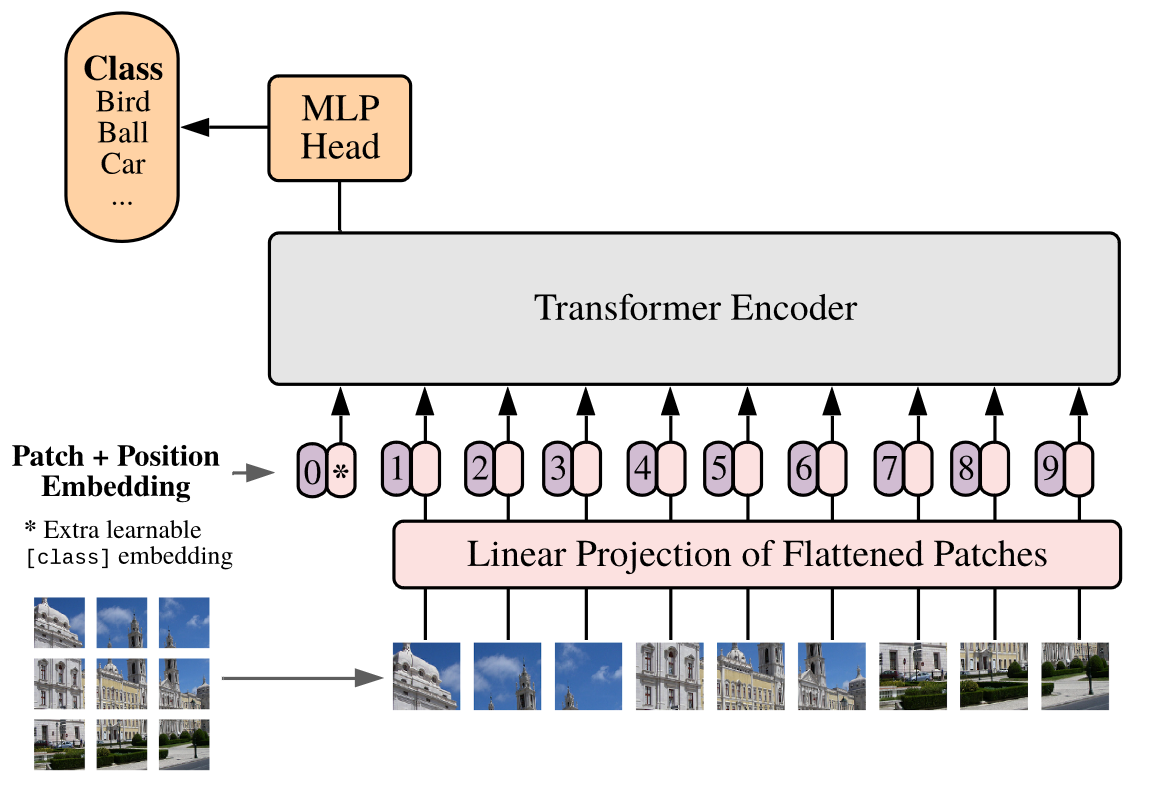
\includegraphics[width=0.9\textwidth]{Images/main/vit_full_arch.png}
	\caption[\textbf{ViT Architecture}]{\textbf{ViT Architecture}. ViT architecture from \cite{dosovitskiy2020image}.}
	\label{fig:vit_full_arch}
\end{figure}

Vision Transformer(ViT) was introduced by Dosovitskiy et al. \cite{dosovitskiy2020image} to overcome the limitations of Convolutional Neural Networks(CNNs) for image recognition. The model applies Transformer architecture to image recognition tasks by treating image patches as sequences of tokens, akin to words in NLP. The highlight of the paper is reusing the transformer encoder from the revolutionary work Vaswani et al.\cite{vaswani2023attentionneed} and adapting to use on images using patch tokenization and positional encoding.

As Cutler uses the features from a self-supervised ViT to generate masks, it is crucial to understand the basics architecture and working of ViT to get a complete picture of the feature generation process. Figure \ref{fig:vit_full_arch} shows the complete architecture of ViT. We are going to go into the main parts of the architecture for a better understanding of the process.

\subsection{Patch Tokens and Positional Encoding}

As each input is an image, unlike sequence of words or tokens in \cite{vaswani2023attentionneed}, the image is divided in fixed size patches(16x16 or 8x8) and each patch is treated as a token and each token is embedded into a fixed-dimensional vector using a learned embedding layer.

\begin{equation}
	\label{eq:pos_encoding}
	z⁰_i = z_i + p_i
\end{equation} 

For each token, instead of using sinusoidal position encodings\cite{vaswani2023attentionneed} to retain information about the position of tokens in the sequence, a learnable position embedding is added as shown in the Eq. \ref{eq:pos_encoding}, where \(p_i \in \mathbb{R}^{D}\) is the learnable position embedding for patch i. 

\begin{equation}
	\label{eq:full_pos_encoding}
	Z = [z_{class}; z⁰_1; z⁰_2;...; z⁰_N]
\end{equation}

Apart from \cite{vaswani2023attentionneed}, ViT\cite{dosovitskiy2020image} introduces a special classification token \(z_{class}\) which is prepended to the sequence of patch embeddings. This token aggregates information from all patches and is used for the final classification task. The final encoding look like Eq. \ref{eq:full_pos_encoding}.

\subsection{Transformer Encoder}
The sequence of patch embeddings, augmented with positional information, is processed by the Transformer encoder. The encoder consists of multiple layers, each comprising Multi-Head Self-Attention (MSA) and Multi-Layer Perceptrons (MLPs), with Layer Normalization (LN) and residual connections.A weighted average\cite{weng2020transformer} of individual attention outputs constitute the final output. Figure \ref{fig:transformer_encoder} illustrates the architecture of transformer encoder. We briefly look into each part.

\begin{figure*}
	\centering
	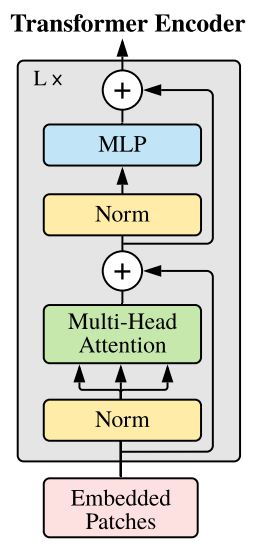
\includegraphics[width=0.3\textwidth]{Images/main/transformerblock.png}
	\caption[\textbf{Transformer Encoder Architecture}]{\textbf{Transformer Encoder Architecture}. Illustration of the Transformer encoder architecture in ViT \cite{dosovitskiy2020image}.}
	\label{fig:transformer_encoder}
\end{figure*}

\subsubsection{Multi-Head Self-Attention (MSA)}
Self-attention allows the model to weigh the importance of different patches relative to each other.

\begin{subequations}
	\label{eq:qkv}
	\begin{align}
		\text{Queries  } Q = zW^{Q}_i \label{eq:query} \\
		\text{Keys  } K= zW^{K}_i \label{eq:key} \\
		\text{Values  } V = zW^{V}_i \label{eq:value}
	\end{align}
\end{subequations}

Given that \(d_k\) is the dimensionality of the key, query, and value vectors and \(W^Q_i, W^K_i, W^V_i \in \mathbb{R}^{D \times d_k }\) are learnable weight matrices, query, key, and value are computed as given in Eq. \ref{eq:qkv}.


For each attention head \(i\),
\begin{equation}
	head_i =
	\text{Attention  }(Q_i,K_i,V_i) = \text{softmax  } \left(\frac{Q_iK^{T}_i}{\sqrt{d_k}}\right)V_i
\end{equation}

The outputs from all heads are concatenated and linearly transformed. Given \(W^O \in \mathbb{R}^{h-d_k \times D } \):
\begin{equation}
	MSA(z) = \text{Concat  }(head_i, head_2..., head_h)W^O
\end{equation}

\subsubsection{Layer Normalization and Residual Connections}
Each layer in the Transformer encoder includes Layer Normalization (LN) and residual (skip) connections
\begin{equation}
	z' = \text{MSA}(\text{LN}(z)) + z
\end{equation}
\begin{equation}
	z'' = \text{MLP}(\text{LN}(z')) + z'
\end{equation}
The Multi-Layer Perceptron (MLP) usually consists of two linear transformations with a GELU non-linearity in between. Assuming \(W_1\) ans \(W_2\) are learnable weight matrices:
\begin{equation}
	\text{MLP}(x) = W_2(\text{GELU}(W_1x))
\end{equation}

\subsubsection{Output Layer}
The final output of the classification token is passed through a linear layer to produce the classification logits. Given \(C\) is the number of classes and \(W_{class} \in \mathbb{R}^{C \times D }\):
\begin{equation}
	\text{logits} = W_{class} \text{ }.\text{ } z''_{class}
\end{equation}
The linear layer projects the final representation of the classification token into the space of class labels.

\section{DINO}
The self-supervised model DINO, introduced by Caron, Mathilde, et al. \cite{caron2021emerging}, achieves remarkable performance that rivals many state-of-the-art Convolutional Networks (CNN) trained with supervision. DINO stands out for its ability to extract features that reveal clear information about semantic segmentation and scene layout within images. This capability distinguishes DINO from supervised Vision Transformers (ViTs) and ConvNets, underscoring its potential for sophisticated computer vision tasks without relying on annotated data.

As we will be using DINO features for producing the pseudo masks in CutLer {\cite{wang2023cut}, we need a basic understanding of DINO architecture and training.

\subsection{Knowledge distillation}
 Knowledge distillation plays a crucial role in training a student model to mimic the behavior and representations learned by a larger teacher model, both of which are ViTs. 
 
\begin{figure*}
	\centering
	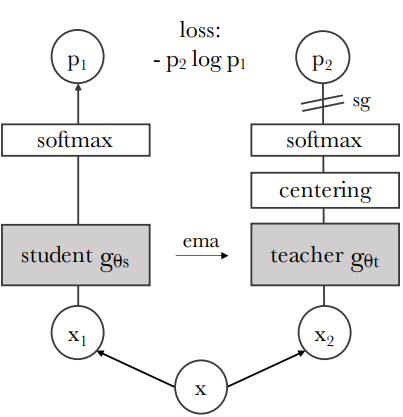
\includegraphics[width=0.5\textwidth]{Images/main/dino.png}
	\caption[\textbf{DINO Architecture }]{\textbf{Architecture of DINO} Illustration provided in 
		\cite{caron2021emerging}.}
	\label{fig:dino}
\end{figure*} 
 
 Initially, the teacher model is typically a ViT that is pre-trained on a large dataset using self-supervised learning techniques. The teacher captures rich, generalized features from the data. The student model is a smaller ViT that aims to replicate the teacher's performance but with fewer parameters, making it computationally lighter and potentially faster during inference.
 
\subsubsection{Momentum Encoder for Teacher}
Instead of using the teacher model directly, DINO employs a momentum encoder mechanism for stability and improved generalization. This means that the parameters of the teacher model are updated using a moving average of the student model's parameters, rather than directly during training.
\begin{equation}
	\label{eq:momentum}
	\theta_t \leftarrow m \theta_t + (1 - m) \theta_s
\end{equation}
The teacher model's parameters are updated using a momentum update rule as given in Eq. \ref{eq:momentum}. Where \(\theta_t\) are the parameters of the teacher model, \(\theta_s\) are the parameters of the student model, and \(m\)is a momentum parameter (typically close to 1) that controls the rate of updating.

\subsection{Training Process}
 DINO uses different augmentations of the same image to create multiple views. These augmented views are passed through both the teacher and student models. Outputs from both models are projected into a lower-dimensional space using projection heads. Outputs from both models are projected into a lower-dimensional space using projection heads. The optimization objective is to minimize the cross-entropy loss between the predicted probability distributions of the teacher and student models. Assume \(P_t(x)\) and \(P_s(x)\) represent the probability distributions predicted by the teacher and student models, respectively. The training process is illustrated in \ref{fig:dino}
 
 \begin{equation}
 	\label{eq:dino_objective}
 	\min_{\theta_s} \mathcal{H}(P_t(x), P_s(x))
 \end{equation}
 
 The cross-entropy loss is computed between the softened distributions of the teacher and student models across all augmented views as given in Eq. \ref{eq:dino_objective}.
 
 \section{CutLer}
 Cutler\cite{wang2023cut} introduces a novel approach to address the challenges of object detection and instance segmentation in an unsupervised learning framework. By integrating Cut-Paste\cite{li2021cutpasteselfsupervisedlearninganomaly} augmentation and a contrastive learning framework, the method not only circumvents the need for labeled data but also achieves state-of-the-art results in object detection and instance segmentation.